\documentclass[border=4pt]{standalone}
\usepackage{mathptmx}
\usepackage[T1]{fontenc}
\usepackage{tikz}
\usetikzlibrary{shapes.geometric,arrows.meta,positioning,fit,calc,backgrounds}
\begin{document}

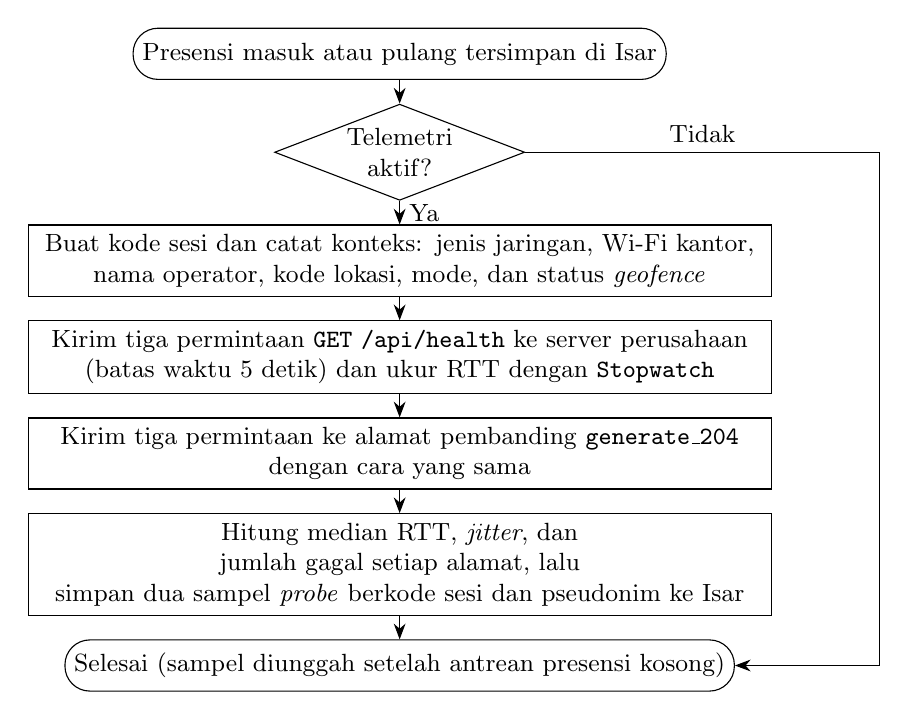
\begin{tikzpicture}[
    node distance=0.30cm,
    proses/.style={rectangle, draw, align=center, text width=9.2cm, minimum height=0.55cm, font=\small},
    batas/.style={rectangle, draw, rounded corners=9pt, align=center, minimum width=2.6cm, minimum height=0.65cm, font=\small},
    keputusan/.style={diamond, draw, aspect=2.6, align=center, inner sep=1pt, font=\small},
    panah/.style={-{Stealth[length=2mm]}}
]
\node[batas] (a) {Presensi masuk atau pulang tersimpan di Isar};
\node[keputusan, below=of a] (k1) {Telemetri\\aktif?};
\node[proses, below=of k1] (b) {Buat kode sesi dan catat konteks: jenis jaringan, Wi-Fi kantor,\\ nama operator, kode lokasi, mode, dan status \textit{geofence}};
\node[proses, below=of b] (c) {Kirim tiga permintaan \texttt{GET /api/health} ke server perusahaan\\ (batas waktu 5 detik) dan ukur RTT dengan \texttt{Stopwatch}};
\node[proses, below=of c] (d) {Kirim tiga permintaan ke alamat pembanding \texttt{generate\_204}\\ dengan cara yang sama};
\node[proses, below=of d] (e) {Hitung median RTT, \textit{jitter}, dan jumlah gagal setiap alamat, lalu\\ simpan dua sampel \textit{probe} berkode sesi dan pseudonim ke Isar};
\node[batas, below=of e] (f) {Selesai (sampel diunggah setelah antrean presensi kosong)};
\draw[panah] (a) -- (k1);
\draw[panah] (k1) -- node[right, font=\small] {Ya} (b);
\draw[panah] (b) -- (c);
\draw[panah] (c) -- (d);
\draw[panah] (d) -- (e);
\draw[panah] (e) -- (f);
\draw[panah] (k1.east) -- node[above, font=\small] {Tidak} ++(4.5,0) |- (f.east);
\end{tikzpicture}
\end{document}
